% Created by tikzDevice version 0.12.3.2 on 2022-02-18 16:30:28
% !TEX encoding = UTF-8 Unicode
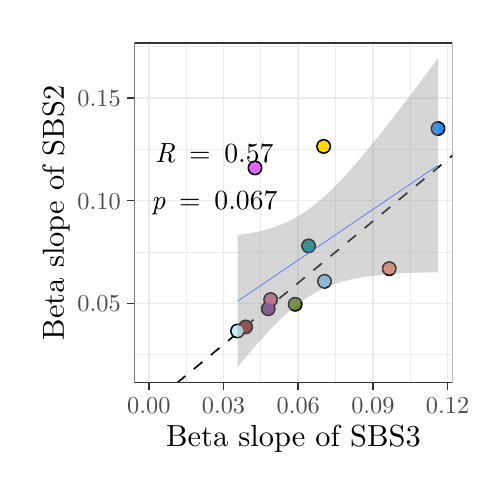
\begin{tikzpicture}[x=1pt,y=1pt]
\definecolor{fillColor}{RGB}{255,255,255}
\path[use as bounding box,fill=fillColor,fill opacity=0.00] (0,0) rectangle (158.99,158.99);
\begin{scope}
\path[clip] (  0.00,  0.00) rectangle (158.99,158.99);
\definecolor{drawColor}{RGB}{255,255,255}
\definecolor{fillColor}{RGB}{255,255,255}

\path[draw=drawColor,line width= 0.6pt,line join=round,line cap=round,fill=fillColor] (  0.00,  0.00) rectangle (158.99,158.99);
\end{scope}
\begin{scope}
\path[clip] ( 38.56, 30.69) rectangle (153.49,153.49);
\definecolor{fillColor}{RGB}{255,255,255}

\path[fill=fillColor] ( 38.56, 30.69) rectangle (153.49,153.49);
\definecolor{drawColor}{gray}{0.92}

\path[draw=drawColor,line width= 0.3pt,line join=round] ( 38.56, 40.78) --
	(153.49, 40.78);

\path[draw=drawColor,line width= 0.3pt,line join=round] ( 38.56, 77.92) --
	(153.49, 77.92);

\path[draw=drawColor,line width= 0.3pt,line join=round] ( 38.56,115.05) --
	(153.49,115.05);

\path[draw=drawColor,line width= 0.3pt,line join=round] ( 38.56,152.18) --
	(153.49,152.18);

\path[draw=drawColor,line width= 0.3pt,line join=round] ( 57.28, 30.69) --
	( 57.28,153.49);

\path[draw=drawColor,line width= 0.3pt,line join=round] ( 84.27, 30.69) --
	( 84.27,153.49);

\path[draw=drawColor,line width= 0.3pt,line join=round] (111.26, 30.69) --
	(111.26,153.49);

\path[draw=drawColor,line width= 0.3pt,line join=round] (138.26, 30.69) --
	(138.26,153.49);

\path[draw=drawColor,line width= 0.6pt,line join=round] ( 38.56, 59.35) --
	(153.49, 59.35);

\path[draw=drawColor,line width= 0.6pt,line join=round] ( 38.56, 96.48) --
	(153.49, 96.48);

\path[draw=drawColor,line width= 0.6pt,line join=round] ( 38.56,133.62) --
	(153.49,133.62);

\path[draw=drawColor,line width= 0.6pt,line join=round] ( 43.78, 30.69) --
	( 43.78,153.49);

\path[draw=drawColor,line width= 0.6pt,line join=round] ( 70.77, 30.69) --
	( 70.77,153.49);

\path[draw=drawColor,line width= 0.6pt,line join=round] ( 97.77, 30.69) --
	( 97.77,153.49);

\path[draw=drawColor,line width= 0.6pt,line join=round] (124.76, 30.69) --
	(124.76,153.49);

\path[draw=drawColor,line width= 0.6pt,line join=round] (151.75, 30.69) --
	(151.75,153.49);
\definecolor{drawColor}{RGB}{0,0,0}

\path[draw=drawColor,line width= 0.6pt,dash pattern=on 4pt off 4pt ,line join=round] ( 16.87,  0.00) -- (158.99,117.31);
\definecolor{fillColor}{RGB}{0,0,0}

\path[draw=drawColor,line width= 0.4pt,line join=round,line cap=round,fill=fillColor] (106.95,116.08) circle (  2.50);

\path[draw=drawColor,line width= 0.4pt,line join=round,line cap=round,fill=fillColor] ( 87.81, 60.74) circle (  2.50);

\path[draw=drawColor,line width= 0.4pt,line join=round,line cap=round,fill=fillColor] (148.27,122.55) circle (  2.50);

\path[draw=drawColor,line width= 0.4pt,line join=round,line cap=round,fill=fillColor] ( 78.77, 50.85) circle (  2.50);

\path[draw=drawColor,line width= 0.4pt,line join=round,line cap=round,fill=fillColor] ( 96.67, 59.03) circle (  2.50);

\path[draw=drawColor,line width= 0.4pt,line join=round,line cap=round,fill=fillColor] (101.49, 80.13) circle (  2.50);

\path[draw=drawColor,line width= 0.4pt,line join=round,line cap=round,fill=fillColor] ( 86.93, 57.40) circle (  2.50);

\path[draw=drawColor,line width= 0.4pt,line join=round,line cap=round,fill=fillColor] ( 82.14,108.32) circle (  2.50);

\path[draw=drawColor,line width= 0.4pt,line join=round,line cap=round,fill=fillColor] (107.26, 67.33) circle (  2.50);

\path[draw=drawColor,line width= 0.4pt,line join=round,line cap=round,fill=fillColor] ( 75.84, 49.39) circle (  2.50);

\path[draw=drawColor,line width= 0.4pt,line join=round,line cap=round,fill=fillColor] (130.65, 71.92) circle (  2.50);
\definecolor{drawColor}{RGB}{255,215,0}
\definecolor{fillColor}{RGB}{255,215,0}

\path[draw=drawColor,line width= 0.4pt,line join=round,line cap=round,fill=fillColor] (106.95,116.08) circle (  1.96);
\definecolor{drawColor}{RGB}{205,96,144}
\definecolor{fillColor}{RGB}{205,96,144}

\path[draw=drawColor,line width= 0.4pt,line join=round,line cap=round,fill=fillColor] ( 87.81, 60.74) circle (  1.96);
\definecolor{drawColor}{RGB}{30,144,255}
\definecolor{fillColor}{RGB}{30,144,255}

\path[draw=drawColor,line width= 0.4pt,line join=round,line cap=round,fill=fillColor] (148.27,122.55) circle (  1.96);
\definecolor{drawColor}{RGB}{139,35,35}
\definecolor{fillColor}{RGB}{139,35,35}

\path[draw=drawColor,line width= 0.4pt,line join=round,line cap=round,fill=fillColor] ( 78.77, 50.85) circle (  1.96);
\definecolor{drawColor}{RGB}{105,139,34}
\definecolor{fillColor}{RGB}{105,139,34}

\path[draw=drawColor,line width= 0.4pt,line join=round,line cap=round,fill=fillColor] ( 96.67, 59.03) circle (  1.96);
\definecolor{drawColor}{RGB}{0,139,139}
\definecolor{fillColor}{RGB}{0,139,139}

\path[draw=drawColor,line width= 0.4pt,line join=round,line cap=round,fill=fillColor] (101.49, 80.13) circle (  1.96);
\definecolor{drawColor}{RGB}{122,55,139}
\definecolor{fillColor}{RGB}{122,55,139}

\path[draw=drawColor,line width= 0.4pt,line join=round,line cap=round,fill=fillColor] ( 86.93, 57.40) circle (  1.96);
\definecolor{drawColor}{RGB}{224,102,255}
\definecolor{fillColor}{RGB}{224,102,255}

\path[draw=drawColor,line width= 0.4pt,line join=round,line cap=round,fill=fillColor] ( 82.14,108.32) circle (  1.96);
\definecolor{drawColor}{RGB}{135,206,250}
\definecolor{fillColor}{RGB}{135,206,250}

\path[draw=drawColor,line width= 0.4pt,line join=round,line cap=round,fill=fillColor] (107.26, 67.33) circle (  1.96);
\definecolor{drawColor}{RGB}{191,239,255}
\definecolor{fillColor}{RGB}{191,239,255}

\path[draw=drawColor,line width= 0.4pt,line join=round,line cap=round,fill=fillColor] ( 75.84, 49.39) circle (  1.96);
\definecolor{drawColor}{RGB}{255,140,105}
\definecolor{fillColor}{RGB}{255,140,105}

\path[draw=drawColor,line width= 0.4pt,line join=round,line cap=round,fill=fillColor] (130.65, 71.92) circle (  1.96);
\definecolor{fillColor}{RGB}{153,153,153}

\path[fill=fillColor,fill opacity=0.40] ( 75.84, 84.04) --
	( 76.75, 84.16) --
	( 77.67, 84.29) --
	( 78.59, 84.43) --
	( 79.50, 84.57) --
	( 80.42, 84.73) --
	( 81.34, 84.90) --
	( 82.26, 85.08) --
	( 83.17, 85.28) --
	( 84.09, 85.49) --
	( 85.01, 85.71) --
	( 85.92, 85.95) --
	( 86.84, 86.20) --
	( 87.76, 86.48) --
	( 88.67, 86.77) --
	( 89.59, 87.08) --
	( 90.51, 87.41) --
	( 91.42, 87.76) --
	( 92.34, 88.14) --
	( 93.26, 88.54) --
	( 94.17, 88.97) --
	( 95.09, 89.42) --
	( 96.01, 89.89) --
	( 96.92, 90.40) --
	( 97.84, 90.93) --
	( 98.76, 91.49) --
	( 99.68, 92.08) --
	(100.59, 92.70) --
	(101.51, 93.34) --
	(102.43, 94.02) --
	(103.34, 94.72) --
	(104.26, 95.45) --
	(105.18, 96.21) --
	(106.09, 97.00) --
	(107.01, 97.81) --
	(107.93, 98.65) --
	(108.84, 99.51) --
	(109.76,100.39) --
	(110.68,101.30) --
	(111.59,102.22) --
	(112.51,103.17) --
	(113.43,104.14) --
	(114.35,105.12) --
	(115.26,106.12) --
	(116.18,107.13) --
	(117.10,108.17) --
	(118.01,109.21) --
	(118.93,110.27) --
	(119.85,111.34) --
	(120.76,112.42) --
	(121.68,113.51) --
	(122.60,114.62) --
	(123.51,115.73) --
	(124.43,116.85) --
	(125.35,117.98) --
	(126.26,119.12) --
	(127.18,120.26) --
	(128.10,121.42) --
	(129.02,122.57) --
	(129.93,123.74) --
	(130.85,124.91) --
	(131.77,126.09) --
	(132.68,127.27) --
	(133.60,128.45) --
	(134.52,129.64) --
	(135.43,130.84) --
	(136.35,132.04) --
	(137.27,133.24) --
	(138.18,134.45) --
	(139.10,135.66) --
	(140.02,136.87) --
	(140.93,138.09) --
	(141.85,139.31) --
	(142.77,140.53) --
	(143.69,141.75) --
	(144.60,142.98) --
	(145.52,144.21) --
	(146.44,145.44) --
	(147.35,146.68) --
	(148.27,147.91) --
	(148.27, 70.59) --
	(147.35, 70.58) --
	(146.44, 70.58) --
	(145.52, 70.56) --
	(144.60, 70.55) --
	(143.69, 70.54) --
	(142.77, 70.52) --
	(141.85, 70.50) --
	(140.93, 70.47) --
	(140.02, 70.45) --
	(139.10, 70.42) --
	(138.18, 70.38) --
	(137.27, 70.35) --
	(136.35, 70.31) --
	(135.43, 70.26) --
	(134.52, 70.21) --
	(133.60, 70.16) --
	(132.68, 70.11) --
	(131.77, 70.04) --
	(130.85, 69.98) --
	(129.93, 69.90) --
	(129.02, 69.83) --
	(128.10, 69.74) --
	(127.18, 69.65) --
	(126.26, 69.55) --
	(125.35, 69.45) --
	(124.43, 69.34) --
	(123.51, 69.21) --
	(122.60, 69.08) --
	(121.68, 68.94) --
	(120.76, 68.79) --
	(119.85, 68.63) --
	(118.93, 68.46) --
	(118.01, 68.28) --
	(117.10, 68.08) --
	(116.18, 67.87) --
	(115.26, 67.64) --
	(114.35, 67.40) --
	(113.43, 67.14) --
	(112.51, 66.86) --
	(111.59, 66.56) --
	(110.68, 66.24) --
	(109.76, 65.91) --
	(108.84, 65.55) --
	(107.93, 65.17) --
	(107.01, 64.76) --
	(106.09, 64.33) --
	(105.18, 63.87) --
	(104.26, 63.39) --
	(103.34, 62.88) --
	(102.43, 62.34) --
	(101.51, 61.77) --
	(100.59, 61.17) --
	( 99.68, 60.55) --
	( 98.76, 59.89) --
	( 97.84, 59.21) --
	( 96.92, 58.50) --
	( 96.01, 57.76) --
	( 95.09, 56.99) --
	( 94.17, 56.20) --
	( 93.26, 55.38) --
	( 92.34, 54.54) --
	( 91.42, 53.68) --
	( 90.51, 52.79) --
	( 89.59, 51.87) --
	( 88.67, 50.94) --
	( 87.76, 49.99) --
	( 86.84, 49.02) --
	( 85.92, 48.03) --
	( 85.01, 47.03) --
	( 84.09, 46.01) --
	( 83.17, 44.98) --
	( 82.26, 43.93) --
	( 81.34, 42.87) --
	( 80.42, 41.79) --
	( 79.50, 40.71) --
	( 78.59, 39.61) --
	( 77.67, 38.51) --
	( 76.75, 37.39) --
	( 75.84, 36.27) --
	cycle;

\path[] ( 75.84, 84.04) --
	( 76.75, 84.16) --
	( 77.67, 84.29) --
	( 78.59, 84.43) --
	( 79.50, 84.57) --
	( 80.42, 84.73) --
	( 81.34, 84.90) --
	( 82.26, 85.08) --
	( 83.17, 85.28) --
	( 84.09, 85.49) --
	( 85.01, 85.71) --
	( 85.92, 85.95) --
	( 86.84, 86.20) --
	( 87.76, 86.48) --
	( 88.67, 86.77) --
	( 89.59, 87.08) --
	( 90.51, 87.41) --
	( 91.42, 87.76) --
	( 92.34, 88.14) --
	( 93.26, 88.54) --
	( 94.17, 88.97) --
	( 95.09, 89.42) --
	( 96.01, 89.89) --
	( 96.92, 90.40) --
	( 97.84, 90.93) --
	( 98.76, 91.49) --
	( 99.68, 92.08) --
	(100.59, 92.70) --
	(101.51, 93.34) --
	(102.43, 94.02) --
	(103.34, 94.72) --
	(104.26, 95.45) --
	(105.18, 96.21) --
	(106.09, 97.00) --
	(107.01, 97.81) --
	(107.93, 98.65) --
	(108.84, 99.51) --
	(109.76,100.39) --
	(110.68,101.30) --
	(111.59,102.22) --
	(112.51,103.17) --
	(113.43,104.14) --
	(114.35,105.12) --
	(115.26,106.12) --
	(116.18,107.13) --
	(117.10,108.17) --
	(118.01,109.21) --
	(118.93,110.27) --
	(119.85,111.34) --
	(120.76,112.42) --
	(121.68,113.51) --
	(122.60,114.62) --
	(123.51,115.73) --
	(124.43,116.85) --
	(125.35,117.98) --
	(126.26,119.12) --
	(127.18,120.26) --
	(128.10,121.42) --
	(129.02,122.57) --
	(129.93,123.74) --
	(130.85,124.91) --
	(131.77,126.09) --
	(132.68,127.27) --
	(133.60,128.45) --
	(134.52,129.64) --
	(135.43,130.84) --
	(136.35,132.04) --
	(137.27,133.24) --
	(138.18,134.45) --
	(139.10,135.66) --
	(140.02,136.87) --
	(140.93,138.09) --
	(141.85,139.31) --
	(142.77,140.53) --
	(143.69,141.75) --
	(144.60,142.98) --
	(145.52,144.21) --
	(146.44,145.44) --
	(147.35,146.68) --
	(148.27,147.91);

\path[] (148.27, 70.59) --
	(147.35, 70.58) --
	(146.44, 70.58) --
	(145.52, 70.56) --
	(144.60, 70.55) --
	(143.69, 70.54) --
	(142.77, 70.52) --
	(141.85, 70.50) --
	(140.93, 70.47) --
	(140.02, 70.45) --
	(139.10, 70.42) --
	(138.18, 70.38) --
	(137.27, 70.35) --
	(136.35, 70.31) --
	(135.43, 70.26) --
	(134.52, 70.21) --
	(133.60, 70.16) --
	(132.68, 70.11) --
	(131.77, 70.04) --
	(130.85, 69.98) --
	(129.93, 69.90) --
	(129.02, 69.83) --
	(128.10, 69.74) --
	(127.18, 69.65) --
	(126.26, 69.55) --
	(125.35, 69.45) --
	(124.43, 69.34) --
	(123.51, 69.21) --
	(122.60, 69.08) --
	(121.68, 68.94) --
	(120.76, 68.79) --
	(119.85, 68.63) --
	(118.93, 68.46) --
	(118.01, 68.28) --
	(117.10, 68.08) --
	(116.18, 67.87) --
	(115.26, 67.64) --
	(114.35, 67.40) --
	(113.43, 67.14) --
	(112.51, 66.86) --
	(111.59, 66.56) --
	(110.68, 66.24) --
	(109.76, 65.91) --
	(108.84, 65.55) --
	(107.93, 65.17) --
	(107.01, 64.76) --
	(106.09, 64.33) --
	(105.18, 63.87) --
	(104.26, 63.39) --
	(103.34, 62.88) --
	(102.43, 62.34) --
	(101.51, 61.77) --
	(100.59, 61.17) --
	( 99.68, 60.55) --
	( 98.76, 59.89) --
	( 97.84, 59.21) --
	( 96.92, 58.50) --
	( 96.01, 57.76) --
	( 95.09, 56.99) --
	( 94.17, 56.20) --
	( 93.26, 55.38) --
	( 92.34, 54.54) --
	( 91.42, 53.68) --
	( 90.51, 52.79) --
	( 89.59, 51.87) --
	( 88.67, 50.94) --
	( 87.76, 49.99) --
	( 86.84, 49.02) --
	( 85.92, 48.03) --
	( 85.01, 47.03) --
	( 84.09, 46.01) --
	( 83.17, 44.98) --
	( 82.26, 43.93) --
	( 81.34, 42.87) --
	( 80.42, 41.79) --
	( 79.50, 40.71) --
	( 78.59, 39.61) --
	( 77.67, 38.51) --
	( 76.75, 37.39) --
	( 75.84, 36.27);
\definecolor{drawColor}{RGB}{51,102,255}

\path[draw=drawColor,line width= 0.2pt,line join=round] ( 75.84, 60.15) --
	( 76.75, 60.78) --
	( 77.67, 61.40) --
	( 78.59, 62.02) --
	( 79.50, 62.64) --
	( 80.42, 63.26) --
	( 81.34, 63.88) --
	( 82.26, 64.50) --
	( 83.17, 65.13) --
	( 84.09, 65.75) --
	( 85.01, 66.37) --
	( 85.92, 66.99) --
	( 86.84, 67.61) --
	( 87.76, 68.23) --
	( 88.67, 68.86) --
	( 89.59, 69.48) --
	( 90.51, 70.10) --
	( 91.42, 70.72) --
	( 92.34, 71.34) --
	( 93.26, 71.96) --
	( 94.17, 72.58) --
	( 95.09, 73.21) --
	( 96.01, 73.83) --
	( 96.92, 74.45) --
	( 97.84, 75.07) --
	( 98.76, 75.69) --
	( 99.68, 76.31) --
	(100.59, 76.93) --
	(101.51, 77.56) --
	(102.43, 78.18) --
	(103.34, 78.80) --
	(104.26, 79.42) --
	(105.18, 80.04) --
	(106.09, 80.66) --
	(107.01, 81.28) --
	(107.93, 81.91) --
	(108.84, 82.53) --
	(109.76, 83.15) --
	(110.68, 83.77) --
	(111.59, 84.39) --
	(112.51, 85.01) --
	(113.43, 85.64) --
	(114.35, 86.26) --
	(115.26, 86.88) --
	(116.18, 87.50) --
	(117.10, 88.12) --
	(118.01, 88.74) --
	(118.93, 89.36) --
	(119.85, 89.99) --
	(120.76, 90.61) --
	(121.68, 91.23) --
	(122.60, 91.85) --
	(123.51, 92.47) --
	(124.43, 93.09) --
	(125.35, 93.71) --
	(126.26, 94.34) --
	(127.18, 94.96) --
	(128.10, 95.58) --
	(129.02, 96.20) --
	(129.93, 96.82) --
	(130.85, 97.44) --
	(131.77, 98.06) --
	(132.68, 98.69) --
	(133.60, 99.31) --
	(134.52, 99.93) --
	(135.43,100.55) --
	(136.35,101.17) --
	(137.27,101.79) --
	(138.18,102.42) --
	(139.10,103.04) --
	(140.02,103.66) --
	(140.93,104.28) --
	(141.85,104.90) --
	(142.77,105.52) --
	(143.69,106.14) --
	(144.60,106.77) --
	(145.52,107.39) --
	(146.44,108.01) --
	(147.35,108.63) --
	(148.27,109.25);
\definecolor{drawColor}{RGB}{0,0,0}

\node[text=drawColor,anchor=base west,inner sep=0pt, outer sep=0pt, scale=  1.00] at ( 46.09,110.12) {\itshape R};

\node[text=drawColor,anchor=base west,inner sep=0pt, outer sep=0pt, scale=  1.00] at ( 53.35,110.12) { };

\node[text=drawColor,anchor=base west,inner sep=0pt, outer sep=0pt, scale=  1.00] at ( 58.33,110.12) {=};

\node[text=drawColor,anchor=base west,inner sep=0pt, outer sep=0pt, scale=  1.00] at ( 66.07,110.12) { };

\node[text=drawColor,anchor=base west,inner sep=0pt, outer sep=0pt, scale=  1.00] at ( 71.05,110.12) {0.57};

\node[text=drawColor,anchor=base west,inner sep=0pt, outer sep=0pt, scale=  1.00] at ( 44.69, 93.29) {\itshape p};

\node[text=drawColor,anchor=base west,inner sep=0pt, outer sep=0pt, scale=  1.00] at ( 49.78, 93.29) { };

\node[text=drawColor,anchor=base west,inner sep=0pt, outer sep=0pt, scale=  1.00] at ( 54.76, 93.29) {=};

\node[text=drawColor,anchor=base west,inner sep=0pt, outer sep=0pt, scale=  1.00] at ( 62.50, 93.29) { };

\node[text=drawColor,anchor=base west,inner sep=0pt, outer sep=0pt, scale=  1.00] at ( 67.48, 93.29) {0.067};
\definecolor{drawColor}{gray}{0.20}

\path[draw=drawColor,line width= 0.6pt,line join=round,line cap=round] ( 38.56, 30.69) rectangle (153.49,153.49);
\end{scope}
\begin{scope}
\path[clip] (  0.00,  0.00) rectangle (158.99,158.99);
\definecolor{drawColor}{gray}{0.30}

\node[text=drawColor,anchor=base east,inner sep=0pt, outer sep=0pt, scale=  0.88] at ( 33.61, 56.32) {0.05};

\node[text=drawColor,anchor=base east,inner sep=0pt, outer sep=0pt, scale=  0.88] at ( 33.61, 93.45) {0.10};

\node[text=drawColor,anchor=base east,inner sep=0pt, outer sep=0pt, scale=  0.88] at ( 33.61,130.59) {0.15};
\end{scope}
\begin{scope}
\path[clip] (  0.00,  0.00) rectangle (158.99,158.99);
\definecolor{drawColor}{gray}{0.20}

\path[draw=drawColor,line width= 0.6pt,line join=round] ( 35.81, 59.35) --
	( 38.56, 59.35);

\path[draw=drawColor,line width= 0.6pt,line join=round] ( 35.81, 96.48) --
	( 38.56, 96.48);

\path[draw=drawColor,line width= 0.6pt,line join=round] ( 35.81,133.62) --
	( 38.56,133.62);
\end{scope}
\begin{scope}
\path[clip] (  0.00,  0.00) rectangle (158.99,158.99);
\definecolor{drawColor}{gray}{0.20}

\path[draw=drawColor,line width= 0.6pt,line join=round] ( 43.78, 27.94) --
	( 43.78, 30.69);

\path[draw=drawColor,line width= 0.6pt,line join=round] ( 70.77, 27.94) --
	( 70.77, 30.69);

\path[draw=drawColor,line width= 0.6pt,line join=round] ( 97.77, 27.94) --
	( 97.77, 30.69);

\path[draw=drawColor,line width= 0.6pt,line join=round] (124.76, 27.94) --
	(124.76, 30.69);

\path[draw=drawColor,line width= 0.6pt,line join=round] (151.75, 27.94) --
	(151.75, 30.69);
\end{scope}
\begin{scope}
\path[clip] (  0.00,  0.00) rectangle (158.99,158.99);
\definecolor{drawColor}{gray}{0.30}

\node[text=drawColor,anchor=base,inner sep=0pt, outer sep=0pt, scale=  0.88] at ( 43.78, 19.68) {0.00};

\node[text=drawColor,anchor=base,inner sep=0pt, outer sep=0pt, scale=  0.88] at ( 70.77, 19.68) {0.03};

\node[text=drawColor,anchor=base,inner sep=0pt, outer sep=0pt, scale=  0.88] at ( 97.77, 19.68) {0.06};

\node[text=drawColor,anchor=base,inner sep=0pt, outer sep=0pt, scale=  0.88] at (124.76, 19.68) {0.09};

\node[text=drawColor,anchor=base,inner sep=0pt, outer sep=0pt, scale=  0.88] at (151.75, 19.68) {0.12};
\end{scope}
\begin{scope}
\path[clip] (  0.00,  0.00) rectangle (158.99,158.99);
\definecolor{drawColor}{RGB}{0,0,0}

\node[text=drawColor,anchor=base,inner sep=0pt, outer sep=0pt, scale=  1.10] at ( 96.02,  7.64) {Beta slope of SBS3};
\end{scope}
\begin{scope}
\path[clip] (  0.00,  0.00) rectangle (158.99,158.99);
\definecolor{drawColor}{RGB}{0,0,0}

\node[text=drawColor,rotate= 90.00,anchor=base,inner sep=0pt, outer sep=0pt, scale=  1.10] at ( 13.08, 92.09) {Beta slope of SBS2};
\end{scope}
\end{tikzpicture}
